
\section{Diagrammi di Nyquist}
Sono una forma di rappresentazione della risposta armonica, definiti sul piano
di Gauss, si ottiene una curva \textit{graduata} in $\omega$, ossia per ogni
punto $\omega$ corrisponderà una coppia di punti sul piano di Gauss.

Il modulo e la fase della funzione $W(j\omega)$ sono quelli ricavati
nell'analisi per i diagrammi di Bode.

Si potrebbe costruire il grafico tabellando tutti i valori per ogni $\omega$,
in alternativa si arriva alla costruzione a partire dai diagrammi di Bode.
Seguono le regole di tracciamento
\begin{enumerate}
 \item Costruire i diagrammi di Bode (con le eventuali correzioni)
 \item $g=0 \Rightarrow W(j0) \in \mathbb{R}$ si partirà da un punto sull'asse
reale di valore $K_B$
\item $W(j\omega)$ abbandona l'asse reale sempre ortogonalmente.
\item $g<0:W(j0) = 0$ il diagramma parte dall'origine \textit{oppure}

$g>0: |W(j0)| = +\infty$ Asintoto dipendente dalla fase iniziale

\item $n-m>0 \Rightarrow W(j\infty) = 0$ Sistema strettamente proprio, la
tangente dipenderà ancora dalla fase $\phase{W(j\infty)}$
\end{enumerate}

Si consideri un sistema del primo ordine
$$
W(s)  = \frac{K_B}{1+s\tau} \qquad
\left\{\begin{aligned}
\tau&>0\\
K_B&>0
\end{aligned}\right.
$$
Facendo riferimento alle figure \ref{fig.amplitude_binomio} per il modulo e
\ref{fig.phase_monomio} per la fase si partirà da un punto sull'asse reale
$K_B$ dato che la fase iniziale è nulla mentre si termina nell'origine con
angolo asintoticamente pari a \SI{-90}{\degree}
\begin{figure}[h]
\centering
\def\KB{3}
\def\TAU{0.5}
\begin{tikzpicture}[
gnuplot def/.append style={prefix={tikz/}}
]
\begin{scope}
\tikzset{
Nyquist grid/.style={black},
}
\NyquistGraph[smooth,samples=81]{-2:4}
{\POAmp{\KB}{\TAU}}{\POArg{\KB}{\TAU}}

\NyquistGrid
\end{scope}

\end{tikzpicture}
\caption{$K_B = \KB,\ \tau=\TAU$}
\end{figure}

La distribuzione di punti non è uniforme lungo la curva, sono in realtà tutti
addensati nel punto iniziale e nell'origine per $\omega\ll\omega_H$ e
$\omega\gg\omega_H$.

Se $K_B$ fosse negativa con $\tau$ positiva si avrebbe il grafico ribaltato nel
secondo quadrante.

\subsubsection{Funzione del secondo ordine}
Si consideri una funzione del secondo ordine
$$
W(s) = \frac{K_B}{1+\frac{2\zeta}{\omega_n}s + \frac{s^2}{\omega_n^2}}
$$
Le figure d'esempio saranno questa volta la
\ref{fig.amplitude_trinomio} per quanto riguarda il modulo e la
\ref{fig.phase_trinomio} per la fase.
\begin{figure}[h]
\centering
\def\KB{1}
\def\ZETA{0.9}
\def\ZETAA{0.2}
\begin{tikzpicture}[
gnuplot def/.append style={prefix={tikz/}}
]
\begin{scope}
\tikzset{
Nyquist grid/.style={black},
}
\NyquistGraph[smooth,samples=81]{-2:4}
{\SOAmp{\KB}{\ZETA}{1}}{\SOArg{\KB}{\ZETA}{1}}

\NyquistGraph[smooth,samples=1250,color=red]{-2:4}
{\SOAmp{\KB}{\ZETAA}{1}}{\SOArg{\KB}{\ZETAA}{1}}

\NyquistGrid
\end{scope}

\end{tikzpicture}
\caption{$\textcolor{blue}{\zeta=\ZETA},\ \textcolor{red}{\zeta=\ZETAA}$}
\end{figure}

La sovraelongazione dovuta a coefficienti di smorzamento $\zeta$ minori di
$\frac{1}{\sqrt{2}}$ tende ad aumentare la distanza della traiettoria
dall'origine.
Al limite per $\zeta\to 0 $ il grafico degenera in una coppia di semirette da
$K_B$ a $+\infty$ e da $-\infty$ a $0$ rispettando la discontinuità dell'angolo.

\newpage
\subsubsection{Polo nell'origine}
\begin{equation}
W(s) = \frac{K_B}{s}
\label{eq.polo_origine}
\end{equation}
Si ha una funzione di trasferimento con un polo nell'origine, facendo
riferimento alla figura \ref{fig.amplitude_origin_pole} per il guadagno e si
considera il segno della fase pari a \SI{-90}{\degree} come ricavato dalla
equazione \ref{eq:fase_polo_origine}


\begin{figure}[h]
\centering
\def\KB{1}
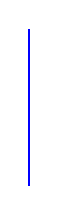
\begin{tikzpicture}[
gnuplot def/.append style={prefix={tikz/}}
]
\begin{scope}
\tikzset{
Nyquist grid/.style={black},
}
%\NyquistGraph[smooth,samples=81]{-2:4}
%{\IntAmp{\KB}}{\IntArg{\KB}}
\draw[color=blue,line width=0.3mm](0,0)--(0,-2);
\NyquistGrid
\end{scope}

\end{tikzpicture}
%\caption{$\textcolor{blue}{\zeta=\ZETA},\ \textcolor{red}{\zeta=\ZETAA}$}
\end{figure}

Esiste in realtà una singolarità nell'origine, si pensa di deformare l'asse
immaginario intorno l'origine con un arco di circonferenza di raggio
$\varepsilon$ ed angolo $\theta\in[0,\frac{\pi}{2}]$, dunque la precedente
equazione \ref{eq.polo_origine} diventa
$$
W(j\omega) = \frac{K_B}{\varepsilon e^{j\theta}}
$$
\begin{figure}[h]
\centering
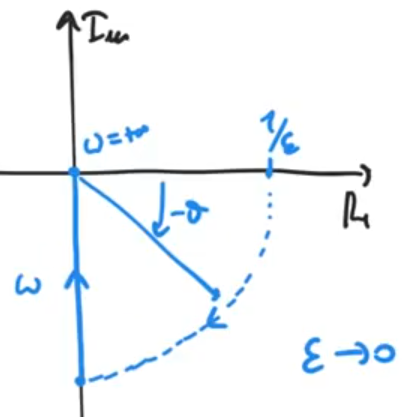
\includegraphics[width=\picwid]{approssimazione_epsilon_polo_origine}
\end{figure}

\subsubsection{Esempio complesso}
Si ha la seguente funzione (in forma di Bode)
$$
W(s) = 10 \frac{1+0.1s}{(1+s)(1+10s)}
$$
Si ricavano i seguenti dati
$$
g=0,\ n-m=1,\ \tau_z=0.1,\ \tau_{p_1}=1,\
\tau_{p_2} = 10,\ K_B = 10
$$

\begin{figure}[h]
\centering
\begin{tikzpicture}[
gnuplot def/.append style={prefix={tikz/}}]
\begin{scope}[xscale=7/3,yscale=3/180]
\tikzset{
semilog lines/.style={black},
}
\OrdBode{15}
\UnitedB
\semilog{-1}{2}{-90}{90}
\BodeGraph[asymp
lines,samples=2000]{-1:2}{\POAmpAsymp{10}{1}+\POAmpAsymp{1}{10}
-\POAmpAsymp{1}{0.1}}

\BodeGraph[samples=100]{-1:2}{\POArg{1}{0.5}}

\end{scope}
\end{tikzpicture}
%\caption{$\textcolor{red}{\tau=<0},\quad
%\textcolor{blue}{\tau=>0} $}
\end{figure}
55:19
